\documentclass[sigplan,10pt,review,anonymous]{acmart}
\settopmatter{printfolios=true,printccs=false,printacmref=false}
\acmConference[PL'18]{ACM SIGPLAN Conference on Programming Languages}{January 01--03, 2018}{New York, NY, USA}
\acmYear{2018}
\acmISBN{} 
\acmDOI{} 
\startPage{1}
\setcopyright{none}
\bibliographystyle{ACM-Reference-Format}

\usepackage{booktabs}  
\usepackage{subcaption} 
\usepackage{amssymb}
\usepackage{stmaryrd}
\usepackage{bbm}
\usepackage[greek,english]{babel}
\usepackage{ucs}
\usepackage[utf8x]{inputenc}
\usepackage{autofe}
\usepackage[references]{agda} 
\usepackage{newunicodechar}
\usepackage[nocenter]{qtree}
\usepackage{tikz}
\usepackage{bbold}
\usetikzlibrary{cd}
\usetikzlibrary{quotes}

\newunicodechar{𝕌}{$\mathbb{U}$}
\newunicodechar{𝔽}{$\mathbb{F}$}
\newunicodechar{𝕋}{$\mathbb{T}$}
\newunicodechar{𝟘}{$\mathbb{0}$}
\newunicodechar{𝟙}{$\mathbb{1}$}
\newunicodechar{𝟚}{$\mathbb{2}$}
\newunicodechar{⋆}{${}_*$}
\newunicodechar{ᵤ}{${}_u$}
\newunicodechar{⊚}{$\fatsemi$}

\newcommand{\alt}{~|~}
\newcommand{\net}{t_\bullet}
\newcommand{\opr}[1]{|#1\rangle\langle#1|}
\newcommand{\inlv}[1]{\ensuremath{\mathit{inl}(v)}}
\newcommand{\inrv}[1]{\ensuremath{\mathit{inr}(v)}}
\newcommand{\ket}[1]{|#1\rangle}
\newcommand{\oneover}[1]{1/#1}
\newcommand{\pointed}[2]{[#1 \bullet #2]}
\newcommand{\nboxtimes}[2]{\,\,~{^{#1}\boxtimes^{#2}}~\,\,}
\newcommand{\mm}{\texttt{\textminus}}
\newcommand{\pp}{\texttt{+}}
\newcommand{\inl}[1]{\textsf{inl}~#1}
\newcommand{\inr}[1]{\textsf{inr}~#1}
\newcommand{\idv}[3]{#2 \xrightarrow{#1} #3}
\newcommand{\cp}[3]{#1\stackrel{#2}{\bullet}#3}
\newcommand{\idt}[3]{#2 \equiv_{#1} #3}
\newcommand{\idrt}[3]{#3 \equiv_{#1} #2}
\newcommand{\refl}[1]{\textsf{refl}~#1}
\newcommand{\lid}{\textsf{lid}}
\newcommand{\rid}{\textsf{rid}}
\newcommand{\linv}{l!}
\newcommand{\rinv}{r!}
\newcommand{\invinv}{!!}
\newcommand{\assoc}{\circ}
\newcommand{\identlp}{\mathit{unite}_+\mathit{l}}
\newcommand{\identrp}{\mathit{uniti}_+\mathit{l}}
\newcommand{\identlsp}{\mathit{unite}_+\mathit{r}}
\newcommand{\identrsp}{\mathit{uniti}_+\mathit{r}}
\newcommand{\swapp}{\mathit{swap}_+}
\newcommand{\assoclp}{\mathit{assocl}_+}
\newcommand{\assocrp}{\mathit{assocr}_+}
\newcommand{\identlt}{\mathit{unite}_*\mathit{l}}
\newcommand{\identrt}{\mathit{uniti}_*\mathit{l}}
\newcommand{\identlst}{\mathit{unite}_*\mathit{r}}
\newcommand{\identrst}{\mathit{uniti}_*\mathit{r}}
\newcommand{\swapt}{\mathit{swap}_*}
\newcommand{\assoclt}{\mathit{assocl}_*}
\newcommand{\assocrt}{\mathit{assocr}_*}
\newcommand{\absorbr}{\mathit{absorbr}}
\newcommand{\absorbl}{\mathit{absorbl}}
\newcommand{\factorzr}{\mathit{factorzr}}
\newcommand{\factorzl}{\mathit{factorzl}}
\newcommand{\dist}{\mathit{dist}}
\newcommand{\factor}{\mathit{factor}}
\newcommand{\distl}{\mathit{distl}}
\newcommand{\factorl}{\mathit{factorl}}
\newcommand{\distz}{\mathit{absorbr}}
\newcommand{\iso}{\leftrightarrow}
\newcommand{\proves}{\vdash}
\newcommand{\idc}{\mathit{id}\!\!\leftrightarrow}
\newcommand{\Rule}[4]{
\makebox{{\rm #1}
$\displaystyle
\frac{\begin{array}{l}#2 \\\end{array}}
{\begin{array}{l}#3      \\\end{array}}$
 #4}}
\newcommand{\jdg}[3]{#2 \proves_{#1} #3}

% 12 pages

%%%%%%%%%%%%%%%%%%%%%%%%%%%%%%%%%%%%%%%%%%%%%%%%%%%%%%%%%%%%%%%%%%%%%%%%%%%
\begin{document}

\title{Fractional Types}
\author{Chao-Hong Chen}
\affiliation{
  \institution{Indiana University}
}

\author{Vikraman Choudhury}
\affiliation{
  \institution{Indiana University}
}

\author{Jacques Carette}
\affiliation{
  \institution{McMaster University}
}

\author{Amr Sabry}
\affiliation{
  \institution{Indiana University}
}

\begin{abstract}
  In reversible and quantum computing, the management of space is
  subject to two broad classes of constraints. First, as is the case
  for general-purpose computation, every allocation must be paired
  with a matching de-allocation. Second, space can only be safely
  de-allocated if its contents are restored to their initial value
  from allocation time. Generally speaking, the state of the art
  provides limited partial solutions that address the first
  constraint by imposing a stack discipline and by leaving the second
  constraint to programmer's assertions.

  We propose a novel approach based on the idea of \emph{fractional
    types}. As a simple intuitive example, allocation of a new boolean
  value initialized to \textsf{false} also creates a value
  $\oneover{\textsf{false}}$ that can be thought of as a garbage
  collection (gc) process specialized to reclaim, and only reclaim,
  storage containing the value $\textsf{false}$. This gc process is a
  first-class entity that can sliced and diced by combining it with
  other gc processes and decomposing it in smaller
  processes.

  Technically, we formalize this idea in the context of a reversible
  language founded on type isomorphisms, prove its fundamental
  correctness properties, and illustrate its expressiveness using a
  wide variety of examples. The development is backed by a
  fully-formalized Agda implementation.
\end{abstract}

\maketitle

\input{latex/PiFracDynCode.tex}

%%%%%%%%%%%%%%%%%%%%%%%%%%%%%%%%%%%%%%%%%%%%%%%%%%%%%%%%%%%%%%%%%%%%%%%%%%%
\section{Introduction}

If quantum field theory is correct (as it so far seems to be) then
information, during any physical process, is neither created nor
destroyed. Landauer~\cite{Landauer:1961,Landauer,bennett1985fundamental},
Bennett~\cite{bennett2010notes,bennett2003notes,Bennett:1973:LRC},
Fredkin~\cite{fredkin1982conservative} and others made compelling
arguments that this physical principle induces a corresponding
computational principle of ``conservation of information.'' This
principle is indeed one of the defining characteristics of quantum
computing and its classical restriction known as reversible computing.

\paragraph*{Quantum and Reversible Computing Based on Type
  Isomorphisms.} The Toffoli gate is known to be universal for
classical reversible circuits~\cite{Toffoli:1980}. Adding just one
gate (the Hadamard gate) produces a universal set of primitives for
quantum circuits~\cite{hadtoffuniv}. The ``only'' difference between
the two circuit models is that quantum circuits can process
superpositions of values (waves) in one step whereas classical
circuits lack this form of parallelism. Most importantly, structurally
the two circuits models are identical and one can derive properties
valid for both families by focusing on the simpler classical model. In
fact, classical reversible computations are often used as
``subroutines'' of quantum computations.

Instead of using the rather low-level circuit model of computation,
one can leverage the full force of type theory and category theory by
expressing reversible classical computations as \emph{isomorphisms
  over finite types}~\cite{Fiore:2004,James:2012:IE:2103656.2103667}
or \emph{equivalences over
  groupoids}~\cite{DBLP:conf/esop/CaretteS16}. This perspective is
similarly universal for reversible computation (and can be extended to
quantum computation~\cite{10.1007/978-3-319-89366-2_19}) but with the
advantage of exposing a rich mathematical structure in reversible
computations that we will exploit to solve the ``ancilla problem''
explained next.

\paragraph*{Temporary Storage using Ancilla Bits.} The universality of
the Toffoli gate for classical reversible computing and of the
universality of the Toffol-Hadamard gates for quantum computing should
not distract from efficiency and safety concerns. The theorems proving
universality (i) assume that temporary storage (often called
\emph{ancilla bits}) may be used~\cite{Toffoli:1980}, and (ii) that
this temporary storage is returned to its initial state before
de-allocation. Indeed if no temporary storage is allowed, the Toffoli
gate is not universal~\cite{DBLP:conf/innovations/AaronsonGS17} and as
would be expected the more temporary storage is allowed, the more
efficient certain computations could become.

More fundamentally, the condition requiring that the temporary storage
is only de-allocated when returned to its initial condition is a
safety condition. Violating this condition destroys the symmetry
between input and output making the circuits not reversible and, in
the quantum model, causes decoherence that may destroy the quantum
state. As reviewed in Sec.~\ref{sec:examples}, ancilla bits have a
number of critical applications and yet are poorly supported in
current reversible and quantum programming languages making them a
common source of bugs.

\paragraph*{Conservation of Information and Negative Entropy.}  
According to the conventional theory of
communication~\cite{Shannon1948}, a type with $N$ values is viewed as
an abstract system that has $N$ distinguishable states where the
amount of information contained in each state is $\log{N}$. This
entropy is a measure of information which materializes itself in
memory or bandwidth requirements when storing or transmitting elements
of this type. Thus a type with 8 elements needs 3 bits of memory for
storage or 3 bits of bandwidth for communication. The logarithmic map
implies that information contained in a composite state is the sum of
the information contained in its constituents. For example, the type
$A \times B$ where $A$ has two elements and $B$ has three elements can
be thought of a composite system consisting of two independent
unrelated subsystems.  Each state of the composite system therefore
contains $\log{(2*3)} = \log{2} + \log{3}$ bits which is the sum of
the information contained in each subsystem. If we could imagine a
\emph{fractional type} $\frac{1}{A}$, this type would introduce
negative entropy. For example, a type with ``cardinality''
$\frac{1}{8}$ has entropy $\log{\frac{1}{8}} = -3$. It is natural to
interpret this negative entropy just like we interpret ``negative
money,'' as a resource (space or bandwidth) to be repaid (reclaimed)
by some other part of the system. Indeed, we will introduce such
fractional types and use them to represent ``garbage collection
processes'' that reclaim temporary storage. Just like in the case of
``negative money'' it is critical that these fractional types be
linearly used, i.e., they cannot be duplicated or erased: this
property is however automatically enforced in a reversible
computational model!

\paragraph*{Outline.} The paper solves the ancilla problem in
reversible and quantum computation using a novel concept:
\emph{fractional types}. In the next section, we introduce the problem
of ancilla, motivate its importance, and explain the limitations of
current solutions. In Sec.~\ref{sec:pi}, we review previous work by
James et al.~\cite{rc2011,rc2012,James:2012:IE:2103656.2103667} that
introduces a reversible programming language built using isomorphism
of types. Although it is conceivable that the concept of fractional
types would apply to general-purpose languages (after some
adaptation), its natural technical definition is using symmetries
present in categorical model of type isomorphisms. We present such a
definition in Sec.~\ref{sec:dyn}: that definition captures the main
ideas of fractional types and partially solves a more general and more
expressive instance of the ancilla problem. The approach however
shares the limitation of current solutions in that it relies on
runtime checks for programmer's assertions that values have been
restored to their initial value before de-allocation. To remedy this
limitation, we refine the type system in Sec.~\ref{sec:dep} to keep
track of values in focus. Technically this requires the introduction
of pointed types on top of which are defined both a monad and co-monad
of singleton types. To justify the claim that fractional types solve
the management of ancilla-based scratch space, we present in
Sec.~\ref{sec:space} an operational semantics that exposes memory
management details using a realization of fractional types as
first-class dependently-typed garbage collectors. In Sec.~\ref{cat} we
present a rich collection of examples illustrating the expressive
power of fractional types. We conclude with a discussion of related
work and a summary of our results. 

%%%%%%%%%%%%%%%%%%%%%%%%%%%%%%%%%%%%%%%%%%%%%%%%%%%%%%%%%%%%%%%%%%%%%%%%%%%
\section{Ancilla Bits}
\label{sec:examples}
 
Restricting a reversible (classical or quantum) circuit to use no
ancillae is like restricting a Turing machine to use no memory other
than the $n$ bits used to represent the
input~\cite{DBLP:conf/innovations/AaronsonGS17}. As such a restriction
disallows countless computations for trivial reasons, reversible and
quantum models of computation have, since their inception, included
management for scratch storage in the form of ancilla
bits~\cite{Toffoli:1980} with the fundamental restriction that such
bits must be returned to their initial states before being safely
reused or de-allocated.

%%%
\subsection{Applications}
 
Beyond computability and efficiency reasons, ancillae have found a
wide range of interesting applications. 

\paragraph*{Quantum blackboxes and Phase Kickback Trick.} Consider a
small database with four elements $a$, $b$, $c$, and $d$. We are given
a function $f$ that maps every element to $0$ except for one element
of interest, e.g., $f(a)=1$ and $f(b)=f(c)=f(d)=0$. In the worst case,
finding the element of interest might require applying $f$ to every
element of the database. In the quantum world we can find the element
much more efficiently using Grover's
algorithm~\cite{Grover:1996:FQM:237814.237866}. We start by building
an equally weighted superposition of the elements:
$\frac{1}{2}\ket{a}+\frac{1}{2}\ket{b}+\frac{1}{2}\ket{c}+\frac{1}{2}\ket{d}$
and operate concurrently of the superposition as follows:

\[\begin{array}{l}
                    \frac{1}{2}\ket{a}+\frac{1}{2}\ket{b}+\frac{1}{2}\ket{c}+\frac{1}{2}\ket{d}\\
\\
\Rightarrow  \textrm{phase kickback} \\
\\
-\frac{1}{2}\ket{a}+\frac{1}{2}\ket{b}+\frac{1}{2}\ket{c}+\frac{1}{2}\ket{d}\\
\\
\Rightarrow  \textrm{diffusion} \\
\\
 (\frac{1}{2}-(-\frac{1}{2}))\ket{a}+(\frac{1}{2}-\frac{1}{2})\ket{b}+(\frac{1}{2}-\frac{1}{2})\ket{c}+(\frac{1}{2}-\frac{1}{2})\ket{d})\\
\\
\Rightarrow  \textrm{simplification} \\
\\
\ket{a}
\end{array}\]

The question, which arises repeatedly in quantum computation, is how
to implement operations such as phase kickback. Essentially we want to
concurrently perform the following action on every element of the
superposition:
\[\begin{array}{l}
  \textbf{if}~\textit{current-element}=\ket{a} \\
  \textbf{then}~\textit{negate} \\
  \textbf{else}~\textit{identity}
\end{array}\]
In the quantum world, na\"\i vely attempting to test whether the
current element is equal to $\ket{a}$ by performing a measurement would
destroy the quantum superposition defeating the entire algorithm.

Here is where ancilla qubits come to the rescue. In the words of
Matuschak and Nielsen~\cite{howgrover}, the idea is the following:
\begin{quote}
  There's a rough heuristic worth noting here, which is that you can
  often convert \verb|if-then| style of thinking into quantum
  circuits. You introduce an ancilla qubit to store the outcome of
  evaluating the \verb|if| condition. And then depending on the state
  of the ancilla, you perform the appropriate state
  manipulation. Finally, when possible you reverse the initial
  computation, resetting the ancilla to its original state so you can
  subsequently ignore it.
\end{quote}

\paragraph*{Quantum Error Correction.} The main requirement for
quantum error correction is the ability to replicate the state of a
qubit onto a number of qubits~\cite[Ch.~3]{NAP25196}. This is however
impossible to do directly by the no-cloning theorem. Again ancilla
qubits come to the rescue: because ancilla qubits start in a known
initial state, it is possible to create a simple circuit that makes
their output state match a protected qubit without knowing or
disturbing the protected qubit. Chong et al.~\cite{sigarchblog}
illustrate the idea with a simple example:
\begin{quote}
consider a 3-qubit quantum majority code in which a logical ``0'' is
encoded as ``000'' and a logical ``1'' is encoded as ``111.''  Just as with
a classical majority code, a single bit-flip error can be corrected by
restoring to the majority value.  Unlike a classical code, however, we
can not directly measure the qubits else their quantum state will be
destroyed.  Instead, we measure syndromes from each possible pair of
qubits by interacting them with an ancilla, then measure each ancilla.
Although the errors to the qubits are actually continuous, the effect
of measuring the ancilla is to discretize the errors, as well as
inform us whether an error occurred so that it can be corrected.  
\end{quote}

\paragraph*{Deferring Quantum Measurements.} The evolution of a
quantum system is deterministic. Measurement add significant
complications, collapsing the quantum state, and producing
probabilistic results. However, using ancilla qubits it is possible to
avoid doing any intermediate measurements in a quantum
circuit~\cite{dewolf}. 

%%%
\subsection{Ancillae Bugs in Benchmarks.}
Despite its fundamental importance, the management of ancillae is
poorly supported in current languages, simulators, and toolkits as
demonstrated in a recent analysis of bugs in quantum
benchmarks~\cite{DBLP:conf/oopsla/HuangM18}. The analysis reveals that
lack of language support in the management of ancillae leads to
several problems. For example: 
\begin{quote}
  \textbf{Bug type 6: Incorrect composition of operations using mirroring}
  Section~4.5 discussed how bugs in deallocating ancillary qubits can
  happen due to bad parameters. Here we see how bugs in deallocating
  ancillary qubits can happen due to incorrect composition of
  operations following a mirroring pattern. For example, in Table~7,
  the operations in rows 2 and 3 are respectively mirrored and undone
  in rows~6 and~5. These lines of code need careful reversal of every
  loop and every operation.
\end{quote}

%%%%%%%%%%%%%%%%%%%%%%%%%%%%%%%%%%%%%%%%%%%%%%%%%%%%%%%%%%%%%%%%%%%%%%%%%%%
\begin{figure*}[t]
\[\begin{array}{rrcll}
\idc :& \tau & \iso & \tau &: \idc \\
\\
\identlp :&  0 + \tau & \iso & \tau &: \identrp \\
\swapp :&  \tau_1 + \tau_2 & \iso & \tau_2 + \tau_1 &: \swapp \\
\assoclp :&  \tau_1 + (\tau_2 + \tau_3) & \iso & (\tau_1 + \tau_2) + \tau_3 &: \assocrp \\
\\
\identlt :&  1 * \tau & \iso & \tau &: \identrt \\
\swapt :&  \tau_1 * \tau_2 & \iso & \tau_2 * \tau_1 &: \swapt \\
\assoclt :&  \tau_1 * (\tau_2 * \tau_3) & \iso & (\tau_1 * \tau_2) * \tau_3 &: \assocrt \\
\\
\distz :&~ 0 * \tau & \iso & 0 ~ &: \factorzl \\
\dist :&~ (\tau_1 + \tau_2) * \tau_3 & \iso & (\tau_1 * \tau_3) + (\tau_2 * \tau_3)~ &: \factor
\end{array}\]
\begin{center}
\Rule{}
{\jdg{}{}{c_1 : \tau_1 \iso \tau_2} \quad \vdash c_2 : \tau_2 \iso \tau_3}
{\jdg{}{}{c_1 \odot c_2 : \tau_1 \iso \tau_3}}
{}
\\
\Rule{}
{\jdg{}{}{c_1 : \tau_1 \iso \tau_2} \quad \vdash c_2 : \tau_3 \iso \tau_4}
{\jdg{}{}{c_1 \oplus c_2 : \tau_1 + \tau_3 \iso \tau_2 + \tau_4}}
{}
\qquad
\Rule{}
{\jdg{}{}{c_1 : \tau_1 \iso \tau_2} \quad \vdash c_2 : \tau_3 \iso \tau_4}
{\jdg{}{}{c_1 \otimes c_2 : \tau_1 * \tau_3 \iso \tau_2 * \tau_4}}
{}
\end{center}
\caption{$\Pi$-terms and combinators.}
\label{pi-terms}
\end{figure*}

\section{Preliminaries: $\Pi$}
\label{sec:pi}

The step from reversible classical circuits to quantum circuits
requires the addition of just one gate that creates
superpositions. Similarly the step from a reversible classical
programming language to a quantum one requires just the management of
superpositions~\cite{10.1007/978-3-319-89366-2_19}. In the cited
paper, the core reversible classical language was Theseus~\cite{XXX},
a language that adds convenient syntactic extensions over an more
basic language $\Pi$ of combinators witnessing isomorphisms over
finite types~\cite{XXX}. The combinator-based language has the
advantage of being convenient for formal analysis for at least two
reasons: (i) it is conceptually simple and small, and (ii) it has
direct and evident connections to type theory and category
theory. Indeed our solution for managing ancillae is inspired by the
construction of \emph{compact closed categories}~\cite{XXX}. These
categories extend the monoidal categories~\cite{XXX} which are to
model most models of resource-aware programming languages~\cite{XXX}
with a new type constructor that creates duals or inverses to existing
types. This will be our fractional type.

%%%%%
\subsection{Core $\Pi$}

The syntax of the language consists of several categories:
\[\begin{array}{lrcl}
\textit{Value types} & t &::=& 0 \alt 1 \alt t+t \alt t*t \\
\textit{Values}      & v &::=& \star \alt \inlv{v} \alt \inrv{v} \alt (v,v) \\
\textit{Level-1 types} &&& t \leftrightarrow t \\
\textit{Level-1 programs} & c &::=& (\textrm{See Fig.~\ref{pi-terms}})\\
\textit{Level-2 types} &&& c \Leftrightarrow c \\
\textit{Level-2 programs} & \alpha &::=& (\textrm{Omitted})
\end{array}\]

Focusing on finite types, the building blocks of type theory are: the
empty type ($0$), the unit type ($1$), the sum type ($+$), and the
product ($\times$) type. One may view each type $A$ as a collection of
physical wires that can transmit $\|A\|$ distinct values where $\|A\|$
is the size of a type, computed as: $\| 0 \| = 0$; $\| 1 \| = 1$;
$\| A + B \| = \| A \| + \| B \|$; and
$\| A \times B \| = \| A \| * \| B \|$. Thus the type
$\mathbb{B} = 1 + 1$ corresponds to a wire that can transmit two
values, i.e., bits, and the type
$\mathbb{B} \times \mathbb{B} \times \mathbb{B}$ corresponds to a
collection of wires that can transmit three bits. From that
perspective, a type isomorphism between types $A$ and $B$ (such that
$\|A\|=\|B\|=n$) models a \emph{reversible} combinational circuit that
\emph{permutes} the $n$ different values. These type isomorphisms are
collected in Fig.~\ref{pi-terms}. It is known that these type
isomorphisms are sound and complete for all permutations on finite
types~\cite{Fiore:2004,fiore-remarks} and hence that they are
\emph{complete} for expressing combinational
circuits~\cite{fredkin1982conservative,James:2012:IE:2103656.2103667,Toffoli:1980}. Algebraically,
these types and combinators form a \emph{commutative semiring} (up to
type isomorphism). Logically they form a superstructural logic
capturing space-time tradeoffs~\cite{superstructural}. Categorically,
they form a \emph{bimonoidal category}~\cite{laplaza72}. 

So far, the types encode conventional data structures, i.e, sets of
values and structured trees of values and the isomorphisms act on such
conventional data structures. Universal computation models however
fundamentally rely on the fact that \emph{programs are (or can be
  encoded as) data}, e.g., a Turing machine can be encoded as a string
that another Turing machine (or even the same machine) can
manipulate. In our setting, we ask whether the type isomorphisms in
Fig.~\ref{pi-terms} can themselves be subject to (higher-level)
reversible deformations? The answer is
yes~\cite{Miller:2003:TBA:775832.775915,DBLP:conf/esop/CaretteS16,DBLP:journals/corr/CockettCS17}. We
only give one example below. (We will require a new level-2 program to
witness coherence of fractional types in Sec.~\ref{sec:dep}.)

\begin{center}
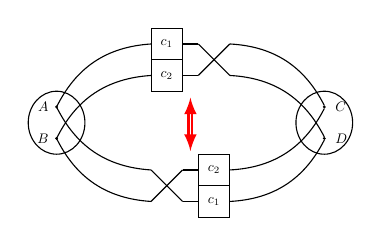
\begin{tikzpicture}[scale=0.4,every node/.style={scale=0.5}]
  \draw[>=latex,<->,double,red,thick] (2.25,-1.2) -- (2.25,-2.9) ;
  \draw (-2,-2) ellipse (0.9cm and 1cm);
  \draw[fill] (-2,-1.5) circle [radius=0.025];
  \node[left] at (-2.1,-1.5) {$A$};
  \draw[fill] (-2,-2.5) circle [radius=0.025];
  \node[left] at (-2.1,-2.5) {$B$};

  \draw (6.5,-2) ellipse (0.9cm and 1cm);
  \draw[fill] (6.5,-1.5) circle [radius=0.025];
  \node[right] at (6.7,-1.5) {$C$};
  \draw[fill] (6.5,-2.5) circle [radius=0.025];
  \node[right] at (6.7,-2.5) {$D$};

  \draw[-] (-2,-1.5) to[bend left] (1,0.5) ;
  \draw[-] (-2,-2.5) to[bend left] (1,-0.5) ;
  \draw[-] (3.5,0.5) to[bend left] (6.5,-1.45) ;
  \draw[-] (3.5,-0.5) to[bend left] (6.5,-2.45) ;

  \draw[-] (-2,-1.5) to[bend right] (1,-3.5) ;
  \draw[-] (-2,-2.5) to[bend right] (1,-4.5) ;
  \draw[-] (3.5,-3.5) to[bend right] (6.5,-1.55) ;
  \draw[-] (3.5,-4.5) to[bend right] (6.5,-2.55) ;

  \draw     (2.5,-3)  -- (3.5,-3) -- (3.5,-4) -- (2.5,-4) -- cycle ;
  \draw     (2.5,-4)  -- (3.5,-4) -- (3.5,-5) -- (2.5,-5) -- cycle ;

  \draw     (1,1)  -- (2,1) -- (2,0) -- (1,0) -- cycle ;
  \draw     (1,0)  -- (2,0) -- (2,-1) -- (1,-1) -- cycle ;

  \node at (3,-3.5) {$c_2$};
  \node at (3,-4.5) {$c_1$};

  \node at (1.5,0.5) {$c_1$};
  \node at (1.5,-0.5) {$c_2$};

  \draw     (2,0.5)  -- (2.5,0.5)  ;
  \draw     (2,-0.5) -- (2.5,-0.5) ;

  \draw     (2.5,0.5)  -- (3.5,-0.5)  ;
  \draw     (2.5,-0.5) -- (3.5,0.5) ;

  \draw     (1,-3.5)  -- (2,-4.5)    ;
  \draw     (1,-4.5) -- (2,-3.5)   ;

  \draw     (2,-3.5)  -- (2.5,-3.5)    ;
  \draw     (2,-4.5) -- (2.5,-4.5)   ;

\end{tikzpicture}
\end{center}

\noindent The top path is the $\Pi$ program
$(c_1~\oplus~c_2)~\odot~\swapp$ which acts on the type $A$ by $c_1$,
acts on the type $B$ by $c_2$, and deforms the resulting space by a
twist that exchanges the two injections into the sum type. The bottom
path performs the twist first and then acts on the type $A$ by $c_1$
and on the type $B$ by $c_2$ as before. If one could imagine the paths
as physical wires and the actions $c_1$ and $c_2$ as permutations on
these wires then, holding the points $A$, $B$, $C$, and $D$ fixed, it
is possible to rotate the top part of the diagram to become identical
to the bottom one. That rotation can be undone (reversed), which takes
the bottom part of the diagram into the top part.  In other words,
there exists a continuous deformation of the program
$(c_1~\oplus~c_2)~\odot~\swapp$ to the program
$\swapp \odot (c_2~\oplus~c_1)$. We can also show that this means
that, as permutations, $(c_1~\oplus~c_2)~\odot~\swapp$ and
$\swapp \odot (c_2~\oplus~c_1)$ are equal. This relation is
non-trivial, as not all programs between the same types can be
deformed into one another. The simplest example of inequivalent
deformations are the two automorphisms of $1+1$, namely $\idc$ and
$\swapp$.

%%%
\subsection{A Small Example}
 
some that ``wants'' ancilla; perhaps fig2b from Dyn. if we want to use
gates with small number of inputs; need to break cccnot to smaller gates



%%%%%%%%%%%%%%%%%%%%%%%%%%%%%%%%%%%%%%%%%%%%%%%%%%%%%%%%%%%%%%%%%%%%%%%%%%%
\section{Interchangeable Ancillae}
\label{sec:dyn}

The management of ancilla data can be teased into two relatively
distinct subproblems:
\begin{itemize}
\item Every allocated ancilla bit must be de-allocated, and 
\item De-allocation of an ancilla bit is only safe if the bit is
  restored to its allocation-time initial value.
\end{itemize}
In this section, we focus on the first subproblem and address the
second in later sections.

%%%%%
\subsection{Scoped Ancilla}

A conventional and efficient way to ensure that every allocation is
paired with a matching de-allocation is to impose a stack
discipline. An illustrative demonstration of this idea is the
\verb|with_ancilla| operator from
Quipper~\cite{Green:2013:QSQ:2491956.2462177}:
\begin{verbatim}
with_ancilla :: (Qubit -> Circ a) -> Circ a
\end{verbatim}
The operator takes a block of gates parameterized by an ancilla,
allocates a new ancilla of type \verb|Qubit| initialized to $\ket{0}$,
and runs the given block of gates. At the end of its execution, the
block is expected to return the ancilla to the state $\ket{0}$ (this
is the second subproblem addressed later) at which point it is
de-allocated. In this scoped-by-construction approach, allocation and
de-allocation of ancillae requires nothing beyond conventional
parameter-passing techniques in which the parameter is allocated
before entry to a function and de-allocated at exit.

This scoped model is therefore quite a pragmatic choice. It is however
limited, and to understand its limitations more vividly, we propose
the following analogy: allocating an ancilla by creating a new wire in
the circuit is like borrowing some money from a global external
entity; the computation has access to a new resource
temporarily. De-allocating the ancilla is like returning the borrowed
money to the global entity; the computation no longer has access to
the additional resource. It would however be unreasonably restrictive
to insist that if the person (function) borrowing the money must be
the same person (function) returning it.
%% , i.e., preventing the following computation:
%% \begin{verbatim}
%%   |-----\  /-----|
%%          \/
%%         / \
%%   |----/   \-----|
%% \end{verbatim}
Indeed, as far as reversible or quantum computation is concerned, the
only important invariant is that information is conserved, i.e., that
money is conserved. The identities of bits or qubits are not
observable as they are all interchangeable in the same way that
particular bills with different serial numbers are interchangeable in
financial transactions. Thus the only invariant is that the net flow
of money between the computation and the global entity is zero. This
observation allows us to go even further than just switching the
identities of borrowers. It is even possible for one person to borrow
\$10, and have three different persons collectively collaborate to
pay back the debt with one person paying \$5, another \$2, and a third
\$3.

Computationally, this extra generality is not a gratuitous concern:
since scope is fundamentally a static property of programs, it does
not allow the flexibility of heap allocation in which the lifetime of
resources is dynamically determined. To summarize, since the
reversible-quantum computational framework guarantees that information
is preserved, it also permits fascinating mechanisms in which
computations can be sliced and diced, decomposed and recomposed, run
forwards and backwards, in arbitrary ways as long as the net balance
is 0.

%%%%%
\subsection{Adding Fractions}
 
We add a new type $\oneover{t}$ with a trivial runtime representation
$\ocircle$. We add two new level-1 programs to introduce and eliminate
the new type, and one new level-2 program that states that
introduction and elimination are inverses:
\[\begin{array}{lrcl}
\textit{Value types} & t &::=& \cdots \alt \oneover{t} \\
\textit{Non-empty types} & \net \\
\textit{Values}      & v &::=& \cdots \alt \ocircle \\
\textit{Level-1 types} &&& t \leftrightarrow t \\
\textit{Level-1 programs} & c &::=& \cdots \alt
   \eta : 1 \leftrightarrow (\net * \oneover{\net}) \\
   &&& ~~~~~\alt \epsilon : (\net * \oneover{\net}) \leftrightarrow 1 \\
\textit{Level-2 types} &&& c \Leftrightarrow c \\
\textit{Level-2 programs} & \alpha &::=& \cdots 
  \alt unity : \epsilon \circ \eta \Leftrightarrow \idc 
\end{array}\]



\EtaEpsilonEval{}

%%%%%
\subsection{Examples}

\EtaEpsilonExamples{}


% of course need de-allocation; keep track of lifetime

% easy: stack but not general

% for general; programmer control or gc

% context of reversible; similar; need allocation; same tradeoffs for
% de-allocation; stack or programmer or gc BUT with caveat. value must
% be restored to its initial value; no information leakage which would
% destroy quantum state

% but reversible also gives you more guarantees; no creation or deletion
% of information means no need to keep track of lifetime of individual
% locations; just need to keep track of ``information''

% General allocation and de-allocation. No need to keep track of
% lifetime. Just make sure location is back to initial value. Safe to
% de-allocate because indistinguishable from freshly created. No pointer
% equality and aliases though. Concurrent: one thread allocates; gc
% thread meets someone else

current proposals for reversible
and quantum programming languages
(e.g. Ricercar~\cite{10.1007/978-3-319-20860-2_13},
Quipper~\cite{Green:2013:QSQ:2491956.2462177}), restrict ancilla bits
to be used in nested scopes, have sound but incomplete laws for
reasoning about the safety condition, and only guarantee safety via
runtime checks.

%%%%%%%%%%%%%%%%%%%%%%%%%%%%%%%%%%%%%%%%%%%%%%%%%%%%%%%%%%%%%%%%%%%%%%%%%%%
\section{Dependently-Typed Garbage Collectors}
\label{sec:dep}

 

We use a Singleton type
to remember this information. 






Formalize ancilla problem in the context of Pi using eta and epsilon
as done in PiFracDyn; more general than scoped; still runtime
check.

When ancilla are created they are created with a specific
value. This value is encoded in the circuit. The value of fractional
type represents the ``garbage collector.''  The garbage collector is
specialized to collect a single value, which is the value used to
create the ancilla value. At this point, if the garbage collector
encounters a different value, it doesn't know what to do, and would
need to throw an exception. This situation in \verb|PiFracDyn| is
similar to current solutions (e.g. Quipper) but actually more general
as it allows non-scoped ancilla allocation and de-allocation. Show
examples.



%%%%% 
\subsection{Pointed Types}
 
%%%%% 
\subsection{Singleton Types}
 
Consider the type $\Sigma \mathbb{N} (\lambda n. n \equiv 5)$. Values
of that type are a number $m$ and a proof that this is number is equal
to 5. So we can have $(4 + 1, \textit{refl})$, $(2 + 3 ,
\textit{refl})$, and so on. All these syntactically different values
are identical to 5 and hence we can \emph{contract} the type to a
single point at 5. 

The denotation of the fractional type is now:

RECIP 

Exploit dependent types to reify proofs in the type system. Type
checking requires (partial) eval. Once we have a proof can we somehow
go back to \verb|PiFracDyn| and remove the runtime check?

Polymorphic type for ancilla?

%%%%%%%%%%%%%%%%%%%%%%%%%%%%%%%%%%%%%%%%%%%%%%%%%%%%%%%%%%%%%%%%%%%%%%%%%%%
\section{Space Operational Semantics}
\label{sec:space}  

Positive rational numbers are a model. Apparently there is a
categorification
\url{https://alistairsavage.ca/pubs/Copelli-Categorification_of_the_Nonnegative_Rational_Numbers.pdf}

Use all the constructions name, coname, etc. and see what they do in this context!

%%%%%%%%%%%%%%%%%%%%%%%%%%%%%%%%%%%%%%%%%%%%%%%%%%%%%%%%%%%%%%%%%%%%%%%%%%%
\section{Trace}
\label{sec:cat}  

Add multiplicative trace, do SAT solver

Toffoli4 using 2 Toffoli3: core of proof of universality; simple
enough. Reversible/Quantum Circuits and Ancilla Wires: Early use of
ancillae in Toffoli's paper to implement arbitrary reversible
functions using a fixed number of 3 input gates
\url{https://link.springer.com/content/pdf/10.1007%2F3-540-10003-2_104.pdf}

In-place matrix transpose: ease of programming, efficiency. Say we
want to transpose a matrix. Wikipedia example
(\url{https://en.wikipedia.org/wiki/In-place_matrix_transposition}):
\begin{verbatim}
11 12 13 14 
21 22 23 24 
\end{verbatim}
transposed to
\begin{verbatim}
11 21
12 22
13 23
14 24
\end{verbatim}
In Pi, the input and output matrices are:
\begin{verbatim}
M = (11,21) , (12,22) , (13,23) , (14,24) 

trM = (11,12,13,14) , (21,22,23,23) 
\end{verbatim}
Say we are given a language like Pi that is sound and complete with
respect to permutations on finite types, we would write the
permutation like so.
\begin{verbatim}
WRITE PERMUTATION
\end{verbatim}
This code does not use additional space, i.e., it performs the matrix
transpose in constant space, i.e., performs an in-place matrix
transposition. It is well know that with additional space, one can
write more efficient matrix transpositions (explain and citations).

Example(s) from Quipper etc. with focus on safety condition. Quipper
uses ancilla bits in several places; one use is to compile
irreversible circuits to reversible ones; need ancilla bits; more
generally several quantum algorithms need ancilla bits (see below); in
quipper de-allocation left to programmer.

Is the below a possible example?

Say we already have a permutation $A \leftrightarrow B$
we can implement a permutation $X \leftrightarrow Z$ 
when there exists $Y$ such that $A = X * Y = Z * Y = B$:
\[\begin{array}{rcl}
X &\rightarrow& X * Y * 1/Y \\
  &\rightarrow& A * 1/Y \\
  &\rightarrow&  B * 1/Y \\
  &\rightarrow&  Y * Z * 1/Y \\
  &\rightarrow&  Z * Y * 1/Y \\
  &\rightarrow&  Z
\end{array}\]
This basically says, in the language of Lens, that
when $A$ is isomorphic to $X \times Y$ and
$B$ is isomorphic to $Z \times Y$, then
$X$ is isomorphic to $Y$.

Another way to think of it: for all isomorphic
$A$ and $B$, whenever they can be factored with a
common complement ($Y$), then the ``other pieces''
(here $X$ and $Y$) are automatically isomorphic.

%%%%%%%%%%%%%%%%%%%%%%%%%%%%%%%%%%%%%%%%%%%%%%%%%%%%%%%%%%%%%%%%%%%%%%%%%%%
\section{Related Work and Conclusion}

%%%%%%%%%%%%%%%%%%%%%%%%%%%%%%%%%%%%%%%%%%%%%%%%%%%%%%%%%%%%%%%%%%%%%%%%%%%
\bibliography{../cites.bib}

\end{document}

%%%%%%%%%%%%%%%%%%%%%%%%%%%%%%%%%%%%%%%%%%%%%%%%%%%%%%%%%%%%%%%%%%%%%%%%%%%
